\documentclass{article}

\usepackage{titlesec}
\usepackage{longtable}
\usepackage{array} % for defining a new column type
\usepackage{varwidth} %for the varwidth minipage environment
\usepackage{color, colortbl}
\usepackage{caption}
\usepackage{subfigure}
\usepackage{filecontents}
\usepackage[section]{placeins}
\usepackage{float}
\usepackage{lscape}

\definecolor{Gray}{gray}{0.9}

\usepackage{pgf-umlsd}
\usepackage{pgf-umlcd}
\newcommand{\sectionbreak}{\clearpage}

\begin{document}

\newcolumntype{M}{>{\begin{varwidth}{4cm}}l<{\end{varwidth}}} %M is for Maximal column

\begin{titlepage}
	\Huge{Bitcode Assignment 1}
\end{titlepage}


\section{The Core}

\subsection{Derive Classes}
For deriving the the right classes that we can implement in the software we firstly look for noun phrases in the requirements document\footnote{https://github.com/mkhattat/bitcode-SEM/blob/master/docs/requirements.pdf}. Secondly we try to refine the list of phrases and group them by using given guidelines.

\paragraph{Noun phrases}
In table \ref{table:ListDerivedNouns} a list of noun phrases is presented that was derived from the functional requirements in the requirements document.

\begin{center}
    \begin{longtable}{ | p{1in} | p{3in} |}
    \hline
    \rowcolor{Gray}
    Noun Phrases & Requirement \\ \hline
    game, board, grid & The game board will consist of a 10x10 square grid \\ \hline
    tile & The game will have six different tiles with which the board will be filled.\\ \hline
    filled board & The game will start with a filled board.\\ \hline
    mouse & A tile must be able to move horizontal or vertical by using the mouse.\\ \hline
    row, column & If one tile is moved, the whole row or column will move along with it. The tiles that get past the edge will reappear at the opposite edge. \\ \hline
	... & A row or column of 3 or more of the same tile (independent of the white outline), will mean that these tiles get removed from the game. \\ \hline
	... & The tiles above empty tiles will move down one position, the remaining empty tiles shall be filled randomly. \\ \hline
	player, move & The game will end when the player runs out of possible moves. \\ \hline
	... & The player should be able to start a new game. \\ \hline
	... & The player should be able to stop a game in progress. \\ \hline
	... & The game shall end when the player loses or stops the game, or clears all of the white outlining. \\ \hline
	turn, cell & The game will end in a set amount of turns. The amount is based upon the amount of cells which are outlined. (For example 1 outlined cell gives the player five moves). \\ \hline
	white outline & Some cells will have a white outline, moving the tile which rests on this cell will not affect the white outline. \\ \hline
	... & The white outlining of a cell will be removed once a tile in that cell is removed. \\ \hline
	pattern & The patterning of white tiles should be preprogrammed. \\ \hline
	... & The player loses when there are no possible moves left, or if the player has run out of moves. \\ \hline
	... & The player wins when all white outlined cells are cleared. \\ \hline
	level, difficulty system & The game could have a level or difficulty based system. \\ \hline
	scoring system & The game could have a scoring system based on the level or difficulty system. \\ \hline
	score & The players score could be shown during the game. \\ \hline
	\caption{list of derived nouns}\label{table:ListDerivedNouns}
    \end{longtable}
\end{center}


\paragraph{Refine Candidates} We can refine the list of nouns by sorting them based on the groups of obvious, uncertain or nonsense class candidates. We also define the type of candidate classes such that it can be a physical object, conceptual entity, categories of classes an interface or values. In table \ref{table:ListCandidateClasses} a list of candidate classes is shown.

\begin{center}
    \begin{longtable}{ | p{1in} | p{1in} | p{2in} |}
    \hline
    \rowcolor{Gray}
    Candidate Class & Group & Class Type \\ \hline
	Game & obvious & conceptual entity \\ \hline
	Board & obvious & interface \\ \hline
	Tile & obvious & conceptual entity \\ \hline
	Mouse & obvious & physical object \\ \hline
	Player & obvious & physical object \\ \hline
	Level & obvious & conceptual entity \\ \hline
	Grid & uncertain & value \\ \hline
	Move & uncertain & conceptual entity \\ \hline
	Pattern & uncertain & value \\ \hline
	ScoringSystem & uncertain & conceptual entity \\ \hline
	Score & uncertain & conceptual entity \\ \hline
	FilledBoard & nonsense & conceptual entity \\ \hline
	Row, Column & nonsense & conceptual entity \\ \hline
	Turn & nonsense & conceptual entity \\ \hline
	WhiteOutline & nonsense & conceptual entity \\ \hline

	\caption{list of candidate classes}\label{table:ListCandidateClasses}
    \end{longtable}
\end{center}


\paragraph{Class-Responsibility-Collaboration Cards} After we refined the list of candidate classes we can create so called "class-responsibility-collaboration Cards" or CRC cards. These cards are used to get an overview of the responsibility of the classes and which classes are collaborating together. In the figure below the CRC cards are presented.

%\documentclass{article}\usepackage{subfigure}\usepackage{float}\begin{document}

\begin{figure}[H]
\begin{subfigure}{}
		\begin{tabular}{|p{1in}|p{1in}|}
			\hline
			\multicolumn{2}{|p{2in}|}{\textbf{Game}} \\ \hline
			\multicolumn{2}{|p{2in}|}{Supperclass(es): ...} \\ \hline
			\multicolumn{2}{|p{2in}|}{Subclasses: ...} \\ \hline
			Create game window	& ... \\ \hline
			Create board & Board \\ \hline
			Create player & Player \\ \hline
		\end{tabular}
		\begin{tabular}{|p{1in}|p{1in}|}
			\hline
			\multicolumn{2}{|p{2in}|}{\textbf{Board}} \\ \hline
			\multicolumn{2}{|p{2in}|}{Supperclass(es): ...} \\ \hline
			\multicolumn{2}{|p{2in}|}{Subclasses: ...} \\ \hline
			Read level & Level \\ \hline
			Create grid & Grid \\ \hline
			Draw board & Tile \\ \hline
			Move Tiles & Move \\ \hline
		\end{tabular}
\end{subfigure}
\begin{subfigure}{}
		\begin{tabular}{|p{1in}|p{1in}|}
			\hline
			\multicolumn{2}{|p{2in}|}{\textbf{Tile}} \\ \hline
			\multicolumn{2}{|p{2in}|}{Supperclass(es): ...} \\ \hline
			\multicolumn{2}{|p{2in}|}{Subclasses: ...} \\ \hline
			Load Image & ... \\ \hline
			Draw Tile & ... \\ \hline
		\end{tabular}
		\begin{tabular}{|p{1in}|p{1in}|}
			\hline
			\multicolumn{2}{|p{2in}|}{\textbf{Move}} \\ \hline
			\multicolumn{2}{|p{2in}|}{Supperclass(es): ...} \\ \hline
			\multicolumn{2}{|p{2in}|}{Subclasses: ...} \\ \hline
			Check for movements & EventHandler \\ \hline
			Move animation & Tile, Grid \\ \hline
		\end{tabular}
\end{subfigure}
\begin{subfigure}{}
		\begin{tabular}{|p{1in}|p{1in}|}
			\hline
			\multicolumn{2}{|p{2in}|}{\textbf{EventHandler}} \\ \hline
			\multicolumn{2}{|p{2in}|}{Supperclass(es): ...} \\ \hline
			\multicolumn{2}{|p{2in}|}{Subclasses: ...} \\ \hline
			Check for mouse events & MouseEvent Handler \\ \hline
			Check for button events & ButtonEvent Handler \\ \hline
		\end{tabular}
		\begin{tabular}{|p{1in}|p{1in}|}
			\hline
			\multicolumn{2}{|p{2in}|}{\textbf{Player}} \\ \hline
			\multicolumn{2}{|p{2in}|}{Supperclass(es): ...} \\ \hline
			\multicolumn{2}{|p{2in}|}{Subclasses: ...} \\ \hline
			keep track of score & ScoringSystem \\ \hline
		\end{tabular}
\end{subfigure}
\begin{subfigure}{}
		\begin{tabular}{|p{1in}|p{1in}|}
			\hline
			\multicolumn{2}{|p{2in}|}{\textbf{MouseEventHandler}} \\ \hline
			\multicolumn{2}{|p{2in}|}{Supperclass(es): ...} \\ \hline
			\multicolumn{2}{|p{2in}|}{Subclasses: ...} \\ \hline
			Capture and handle mouse events & ... \\ \hline
		\end{tabular}
		\begin{tabular}{|p{1in}|p{1in}|}
			\hline
			\multicolumn{2}{|p{2in}|}{\textbf{ButtonEventHandler}} \\ \hline
			\multicolumn{2}{|p{2in}|}{Supperclass(es): ...} \\ \hline
			\multicolumn{2}{|p{2in}|}{Subclasses: ...} \\ \hline
			Capture and handle button events & ... \\ \hline
		\end{tabular}
\end{subfigure}
\begin{subfigure}{}		
		\begin{tabular}{|p{1in}|p{1in}|}
			\hline
			\multicolumn{2}{|p{2in}|}{\textbf{ScoringSystem}} \\ \hline
			\multicolumn{2}{|p{2in}|}{Supperclass(es): ...} \\ \hline
			\multicolumn{2}{|p{2in}|}{Subclasses: ...} \\ \hline
			Keep track of scoring & Move \\ \hline
		\end{tabular}
		\begin{tabular}{|p{1in}|p{1in}|}
			\hline
			\multicolumn{2}{|p{2in}|}{\textbf{Level}} \\ \hline
			\multicolumn{2}{|p{2in}|}{Supperclass(es): ...} \\ \hline
			\multicolumn{2}{|p{2in}|}{Subclasses: ...} \\ \hline
			Read Level from file & ... \\ \hline
		\end{tabular}
\end{subfigure}

\end{figure}
%\end{document}

\paragraph{Comparison with the implementation} If we look at classes that were integrated into the initial implementation of the game\footnote{https://github.com/mkhattat/bitcode-SEM/releases} we can spot some differences. Namely, there are a couple of classes missing. This is mostly due to the fact that not all requirements where implemented in the initial version. For example, the Player class and the ScoringSystem class is absence from the code because scoring is not implemented. There is also not a Level class because there exists only one level that is randomly generated. Furthermore, the Game class is replaced by the Launcher class and Move class is replaced by the Animation class.


\subsection{Main Classes}
Our ‘main’ classes consist of the necessary objects to the core function of the game:
Items, Board, backgorundTileCatalog and the MainScreen. These are the followings:

\paragraph{ItemFactory} his class is responsible for creating random Item classes. This is important mainly because when the items are moved on the board, another random Item should be replaced on the board. These are basically all the pictures we used in for the game, whose point is to make sure 3 or more are set vertically or horizontally and the game has makes sure that after each move there are not any items that can be set in a group of 3 or more.

\paragraph{Board} This class contains everything necessary for the board in our game, it mainly interact with the class Items,  we make sure here that every time a move is made, the items next to each other are not of the same object. If so automatically remove any items (3 or more) next to each other. This class is also responsible for other important tasks namely, creating a random board, replacing and removing items on the board data structure and also finding the similar items on the board.


\paragraph{backgroundTileCatolog} This class contains of an arraylist which holds the position for each tile. We can add a new background tile or remove an existing one, we can count the number of tiles we have added to the arraylist, or check to see if at some given position a background tile already exist or not.( This class works heavily with the Board class, making sure there is always a tile so there won’t be any empty place in our board.)


\paragraph{MainScreen} The MainScreen interacts with all of the other main classes, since it’s responsible for displaying everything and it needs information such as Item, Size of the board, and Tiles to know where everything is and make sure if 3 or more items of the same shape are next to each other automatically remove, also makes sure that the board data structure is in sync with what on the screen is.



\paragraph{MouseEventHandler}  It has one important responsibility and that is capturing the input namely, mouse movements. This class works with animation class and makes sure that moving items on the screen is possible.

\subsection{Reflect on main class decisions}
We consider the other classes as less important since they’re not required for the main function of the game; ScoreCounter makes the game more intersecting (if you reach a certain score you can  update or upgrade to be able to remove more tiles at the same time), but even without the ScoreCounter you should be able to play the game without any problems.
While these functions could likely be handled by the MainScreen class, making them into different classes allows the MainScreen class to be more focused solely on handling rendering tasks, prevents it from becoming bloated, and allows for easier expansion of the functions of ScoreCounting and other functions.

\subsection{The Class diagram}
\begin{figure}[H]
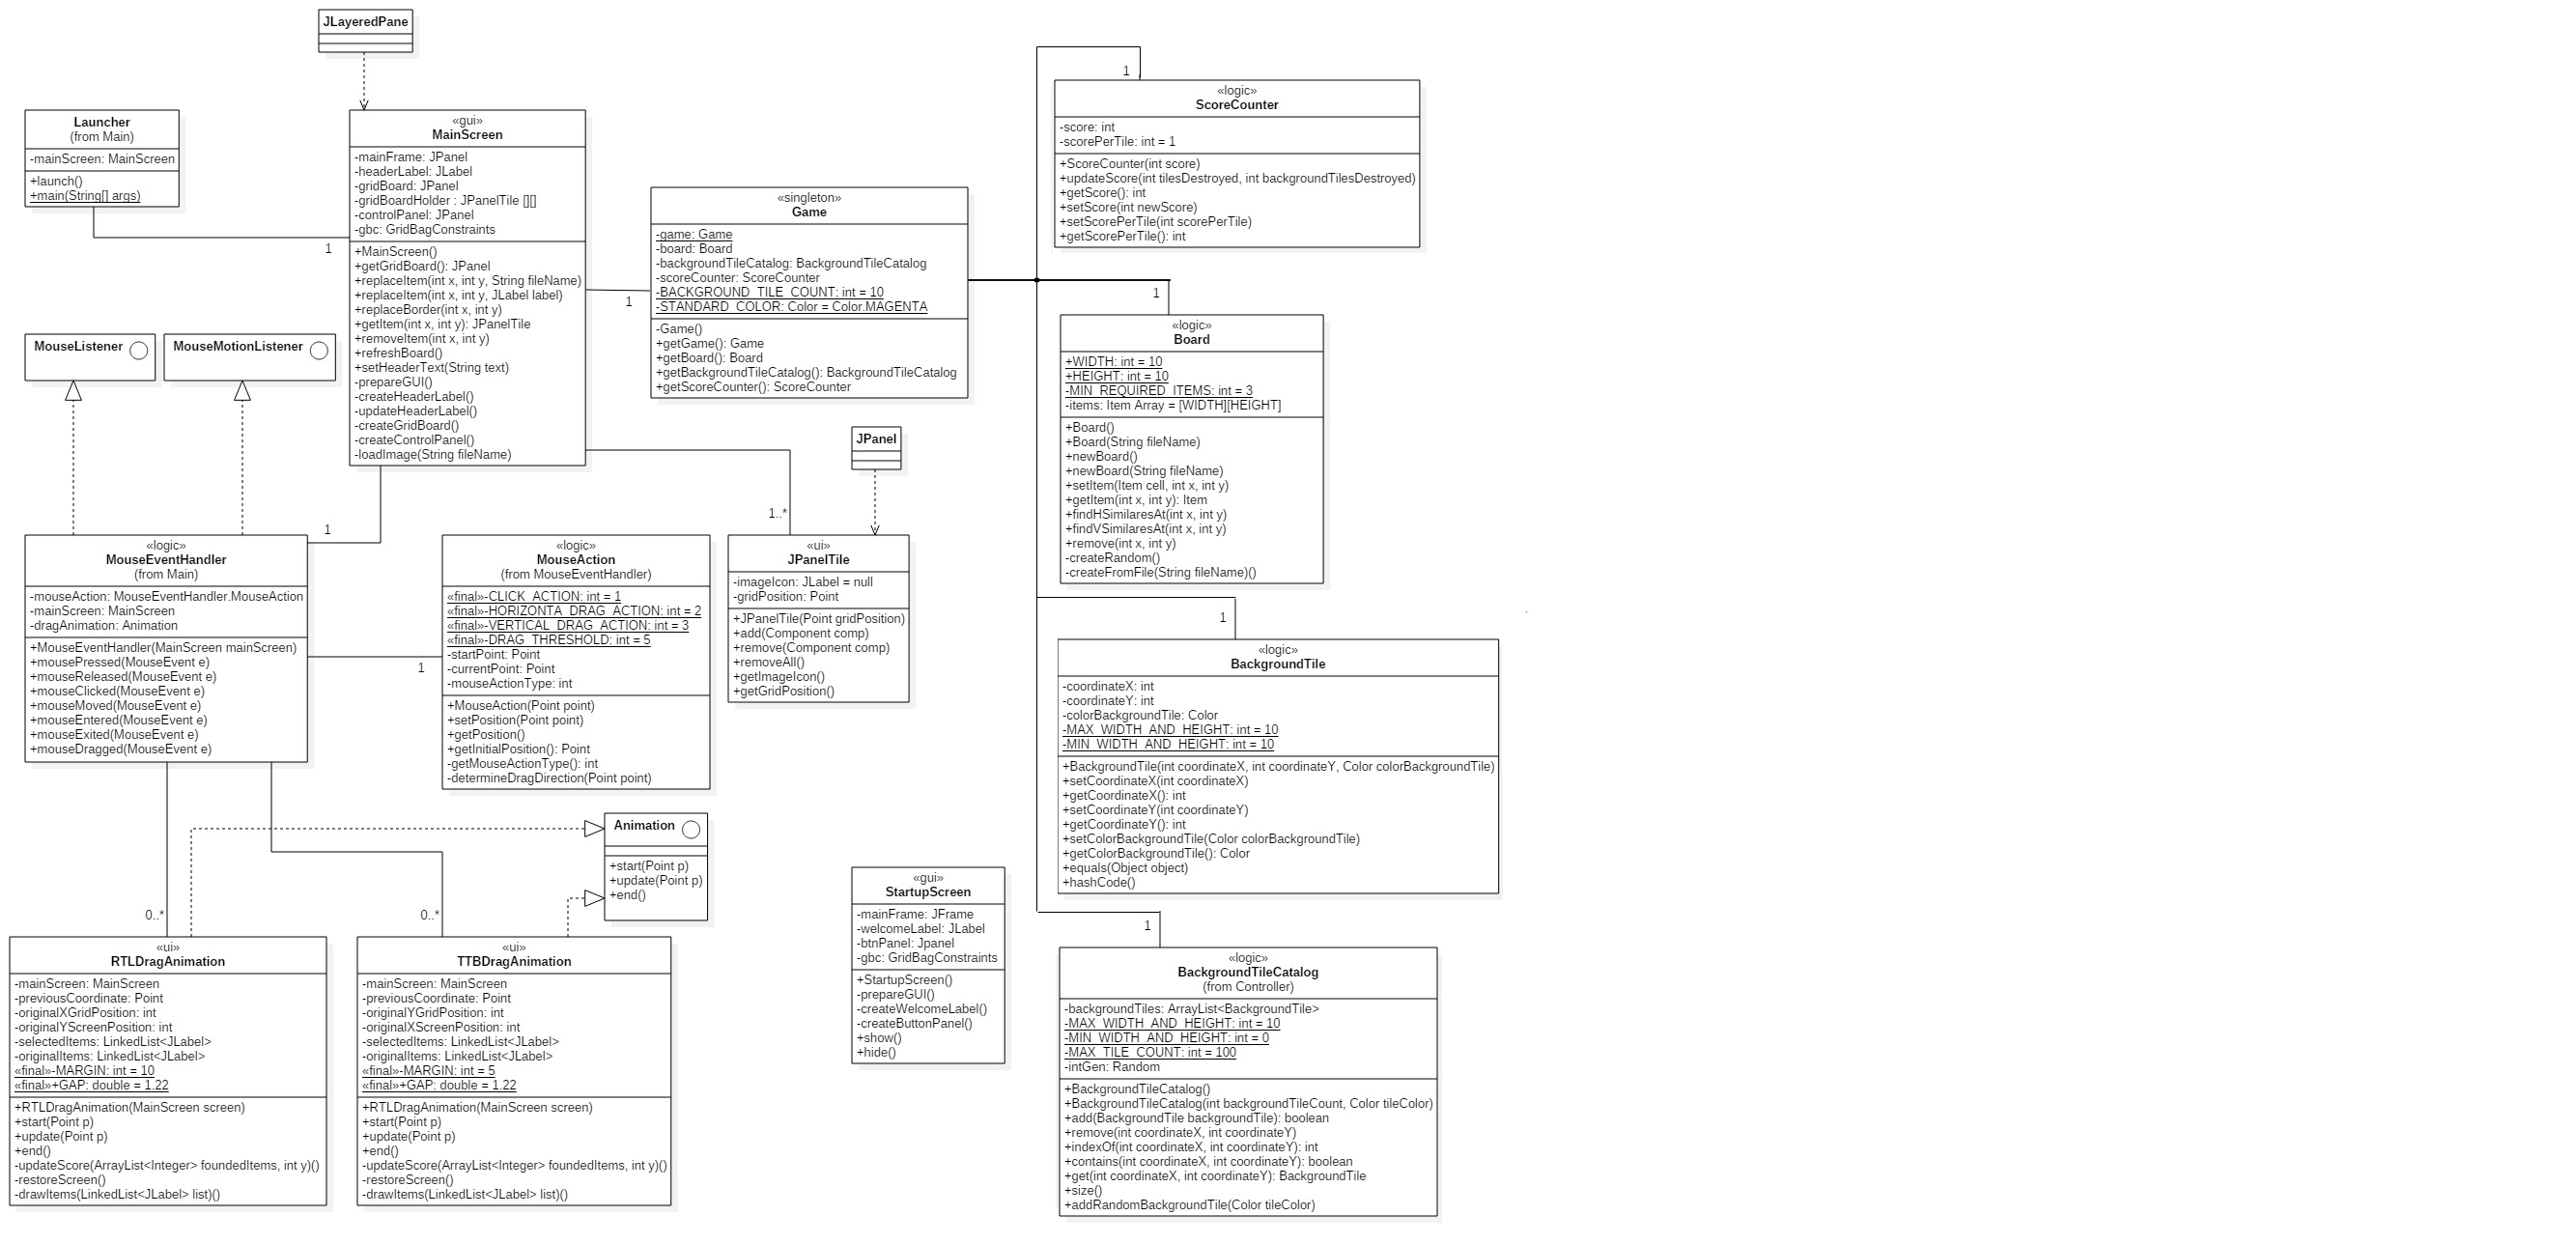
\includegraphics[scale=0.30]{Images/ClassDiagram.png} 
\end{figure}

\subsection{The Sequence Diagram}
\begin{figure}[H]
	\centering
	\begin{sequencediagram}
		\newthread{A}{User}{}
		\newthread{B}{Window/EventHandler}{}
		\newthread{C}{Game}{}
		\newthread{D}{Board}{}
		\begin{call}{A}{Drag Item}{B}{}
			\begin{call}{B}{Check for triples}{C}{}
				\begin{call}{C}{Check for triples}{D}{}
					\begin{sdblock}{Recursion}{}
						\begin{call}{D}{Check for triples}{D}{}
						\end{call}
					\end{sdblock}
				\end{call}
			\end{call}
		\end{call}
	\end{sequencediagram}
\end{figure}

\newpage
\section{UML in Practice}

\subsection{Composition and Aggregation}
\begin{figure}[H]
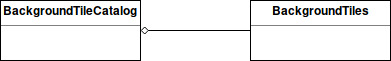
\includegraphics[scale=0.95]{Images/BackgroundTileCatalog.jpg}
An instance of BackgroundTileCatalog contains a reference to the BackgroundTiles class but they are independent and they have their own lifetime, So BackgroundTileCatalog aggregates BackgroundTiles.
\end{figure}

\begin{figure}[H]
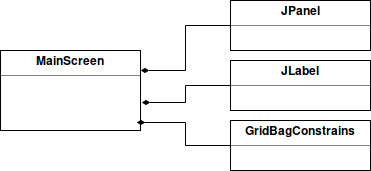
\includegraphics[scale=1]{Images/MainScreen.jpg} 
An instance of MainScreen class has a strong relation, or in other words owns, the JPanel, JLabel, GridBagConstrains classes. There is no reason for these classes to exist without MainScreen class. So it's composition.
\end{figure}

\begin{figure}[H]
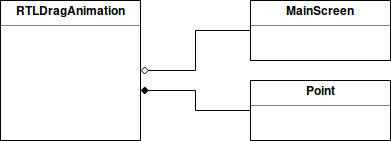
\includegraphics[scale=0.95]{Images/RTLDragAnimation.jpg} 
An instance of RTLDragAnimation class has a relationship with MainScreen and it's aggregation because MainScreen can exist without RTLDragAnimation but at the same time this class owns a Point which cannot exist without RTLDragAnimation, so it's composition.
\end{figure}

\begin{figure}[H]
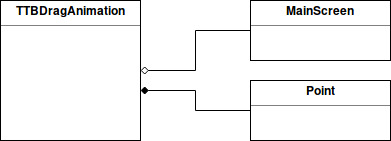
\includegraphics[scale=0.95]{Images/TTBDragAnimation.jpg} 
An instance of TTBDragAnimation class has a relationship with MainScreen and it's aggregation because MainScreen can exist without TTBDragAnimation but at the same time this class owns a Point which cannot exist without TTBDragAnimation, so it's composition.
\end{figure}

\begin{figure}[H]
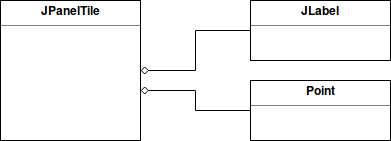
\includegraphics[scale=0.95]{Images/JPanelTile.jpg} 
An instance of JPanelTile class has a relationship with JLabel and Point. It's aggregation because these two classes can exist without JPanelTile.
\end{figure}

\begin{figure}[H]
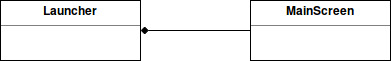
\includegraphics[scale=0.95]{Images/Launcher.jpg} 
A Launcher class owns a MainScreen class because if the Launcher class is killed the MainScreen class will also be killed, so a composition.
\end{figure}

\begin{figure}[H]
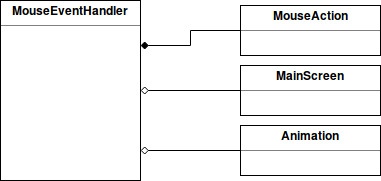
\includegraphics[scale=0.97]{Images/MouseEventHandler.jpg} 
MouseEventHandler aggregates MainScreen and Animation classes. It has a relation with these two classes but they are independent of each other, or in other words an aggregation. But it has a stronger relation with MouseAction, means when MouseEventHandler goes out of scope, then MouseAction also goes out of scope, so in this case a composition.
\end{figure}

\begin{figure}[H]
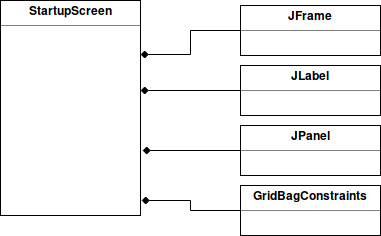
\includegraphics[scale=0.95]{Images/StartupScreen.jpg} 
StartupScreen class owns some classes namely: JFrame, JLabel, JPanel and GridBagConstraints. These classes are dependent on the StartupScreen, means if it dies these classes will also die. So it is a composition.
\end{figure}

\begin{figure}[H]
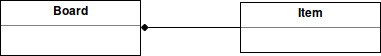
\includegraphics[scale=0.95]{Images/Board.jpg} 
Board class owns an Item class. This is a composition.
\end{figure}

\begin{figure}[H]
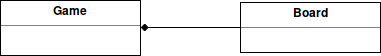
\includegraphics[scale=0.95]{Images/Game.jpg} 
Game class owns a Board class. This is a composition.
\end{figure}

\subsection{Parametrized Classes}
We didn't create any parametrized class in our source code but we use some parametrized classes from standard java library namely ArrayList and LinkedList. Java is a typed language and the concept of parametrized classes is mainly useful for working with collections. Parametrized classes allow us to derive the type of a class. We write the body of a parametrized class, we may invoke some operation on the parameter. Later when the class is bounded with a parameter the compiler tries to ensure this parameter supports operations required by the template.

\subsection{Hierarchy Class Diagrams}
\begin{figure}[H]
	\centering
	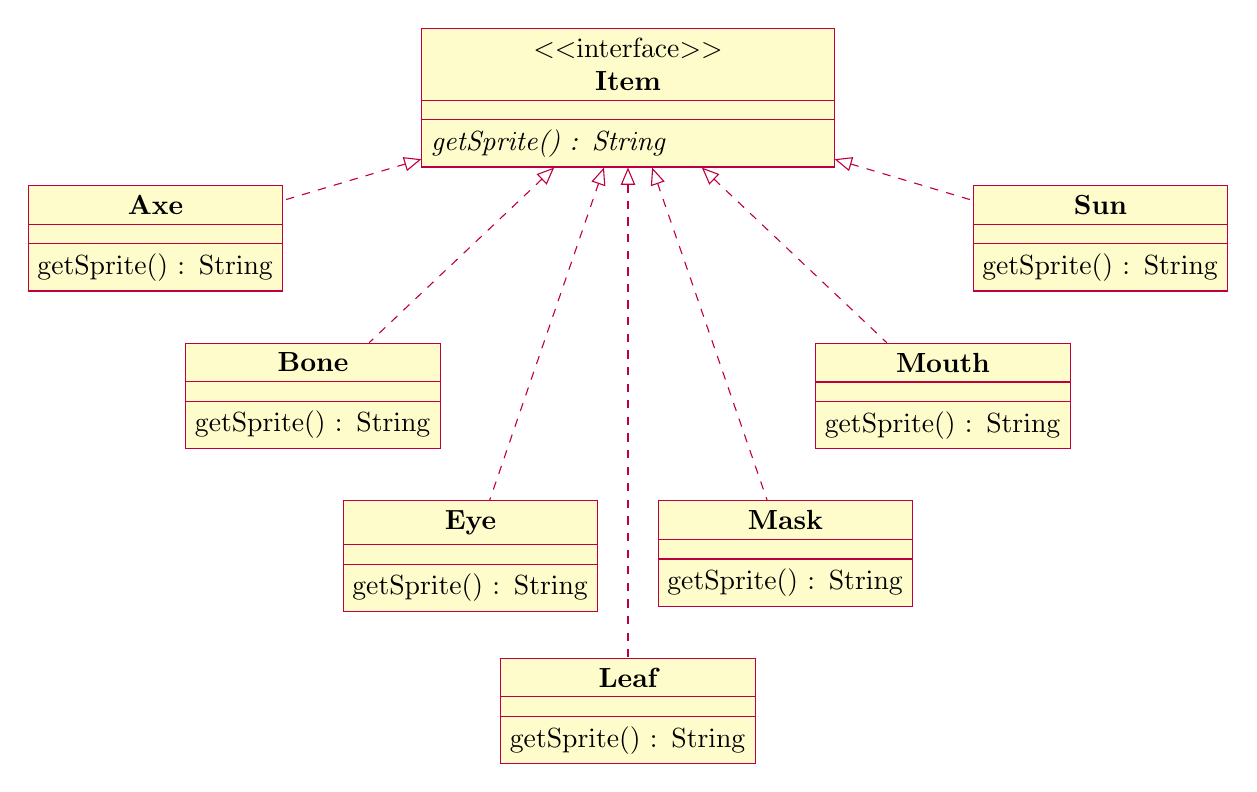
\begin{tikzpicture}
	\begin{interface}{Item}{0,0}
	\operation[0]{getSprite() : String}
	\end{interface}
	\begin{class}[text width = 3cm]{Axe}{-6,-2}
	\implement{Item}
	\operation{getSprite() : String}
	\end{class}
	\begin{class}[text width = 3cm]{Bone}{-4,-4}
	\implement{Item}
	\operation{getSprite() : String}
	\end{class}
	\begin{class}[text width = 3cm]{Eye}{-2,-6}
	\implement{Item}
	\operation{getSprite() : String}
	\end{class}
	\begin{class}[text width = 3cm]{Leaf}{0,-8}
	\implement{Item}
	\operation{getSprite() : String}
	\end{class}
	\begin{class}[text width = 3cm]{Mask}{2,-6}
	\implement{Item}
	\operation{getSprite() : String}
	\end{class}
	\begin{class}[text width = 3cm]{Mouth}{4,-4}
	\implement{Item}
	\operation{getSprite() : String}
	\end{class}
	\begin{class}[text width = 3cm]{Sun}{6,-2}
	\implement{Item}
	\operation{getSprite() : String}
	\end{class}
	\end{tikzpicture}
\end{figure}

Items are produced by an item factory, which can create each of the seven types of items.
Each item implements the item interface, as a result the board can contain every type of item and request its sprite.
A similar functionality could be implemented using an item class with an id attribute, however such an implementation would make further expanding each item individually much more complicated and inconvenient.

\newpage
\section{Traceability}

\subsection{Traceability Strategy}
We have chosen to use a combination of knowledge based and structural based traceability links. We want to use structural based traceability links as much as possible because we think that the code should speak for itself. This means that the links between components in the code should be clear and well defined, also the naming of the artefacts should be consistent. A solution to that is to use tags throughout the documentation:
\begin{itemize}
    \item REQ1: The first requirement
    \item CL1.1-CL1.n: The classes that implement the first requirement
    \item CD1.1-CD1.n: The class diagrams that defines the relations between the classes.
    \item SD1.1-SD1.n: The sequence diagrams that define the sequence of the first requirement
    \item TC1.1-TC1.n: The test cases that test the implementation of the first requirement 
\end{itemize}

\paragraph{} To keep track of traceability links between our code, tests and requirements we have chosen to use a tool called concordion. Concordion can link requirements, unit tests and class implementations by using tags inside de java code. For every requirement there must be a text file that explains the requirement and what should be tested (acceptance testing). To link the requirements and the unit tests a so called fixture java class is created that will be executed when a maven job is ran. After the job is finished a html page is created with the requirements and the test results.

\newpage
\subsection{Traceability Matrix}

\begin{center}
    \begin{longtable}{|p{0.4in}|p{0.4in}|p{0.4in}|p{0.4in}|p{0.4in}|p{0.4in}|p{0.4in}|}
    \hline
             & REQ1 CD1 & REQ1 SD1 & REQ1 CL1.1 & REQ1 CL1.2 & REQ1 TC1.1 & REQ1 TC1.2 \\ \hline
    REQ1 CD1 &    x    &    x     &     x      &     x      &            &            \\ \hline
    REQ1 SD1 &    x    &    x     &     x      &     x      &            &            \\ \hline
    REQ1 CL1.1 &   x     &   x      &    x       &            &      x      &            \\ \hline
    REQ1 CL1.2 &   x     &   x      &            &     x      &            &     x     \\ \hline
    REQ1 TC1.1 &         &          &    x       &            &      x     &            \\ \hline
    REQ1 TC1.2 &         &          &            &     x      &            &     x      \\ \hline
	
	\end{longtable}	
\end{center}


\end{document}






